% !TEX root = main.tex
\section{Systematic uncertainties}
\label{sec:Systematics}

The systematic uncertainties on the measured observables are summarized in Table \ref{tab:normSys} for the decay-time fit to $B_s \to D_s \pi\pi\pi$,
in Table \ref{tab:sigSys} for the decay-time fit to $B_s \to D_s K\pi\pi$
and in Table \ref{tab:sigSys2} for the full time-dependent amplitude fit to $B_s \to D_s K\pi\pi$ decays.
A description of each systematic
effect is given in the following subsections
starting with the ones common to all fits.
Afterwards, systematic effect specific to the amplitude description are discussed.

%This section covers all relevant systematic uncertainties on the measured observables.
%In particular, the model dependent description of the invariant $\Bs$ mass spectrum, the parametrization of the time acceptance using cubic splines, 
%as well as the scaling of the time resolution and tagging calibration are potential sources of systematic errors. 
%The largest contribution of systematic uncertainty is expected to appear in the choice of amplitudes entering the model to describe the 5 dimensional phase space, discussed in Section \ref{sec:fullFit}.

\subsection{Fit bias}
\label{subsec:SystFit}

Pseudo-experiments are performed, where a signal toy sample of the same size as the number of observed signal data events is generated according to the nominal fit model 
and subsequently fitted with the same model.
The means of the pull distributions are taken as systematic uncertainties of the fit parameters.

\subsection{Background subtraction}
\label{subsec:SystMass}

The statistical subtraction of the residual background \cite{Pivk:2004ty}, left after the full selection, relies on the correct description of the invariant $\Bs$ mass distribution.
Since the choice of signal and background models is not unique, alternative parameterizations are tested:

\begin{itemize}

\item The \textsf{Johnson's SU} function which is used as nominal signal model is replaced by the sum of two \textsf{Crystal Ball} functions \cite{CB}. 

\item For the combinatorial background, the nominal second order polynomial is replaced by an exponential function. 

\item For the description of the partially reconstructed background, 
a combination of the \textsf{RooHILLdini} and \textsf{RooHORNsdini} model \cite{Hill:2253246} is used instead of the nominal model of three bifurcated gaussians. 

\item For the shape of the mis-ID background, 
the nominal approach is to use a simulated sample of $\Bs\to\Ds^{-}\pip\pim\pip$ or $\Bs\to\Ds^{*-}\pip\pim\pip$ 
decays and flip the mass hypothesis of the $\pip$ with the higher misidentification probability (see Sec. \ref{sec:massFits}). 
%The resulting $m(\Ds^{(*)}\pion_{\kaon}\pion\pion)$ distribution is then modeled and the shape obtained from the fit is used in the nominal mass fit to signal. 
Two alternative approaches are considered:
we flip the mass hypothesis of the $\pip$ candidate with the lower probability of beeing misidentified; we randomly flip the mass hypothesis of a $\pip$ candidate.

\end{itemize}
%The crystal ball model is given by a gaussian core with an exponential tail on one side. 
%Choosing a double Crystal Ball allows for asymmetric tails in a slightly different way compared to the Johnson's SU function. 
%The HORNSdini model is used to describe the $\Bs\to\Ds^{*}[\to\Ds(\piz)] X_{s/d}$ decay, where the brackets around the $\piz$ indicate that it is missed in the reconstruction. 
%The $\Ds^{*}\to\Ds\piz$ decay is a Vector $\to$ Scalar-Scalar ($1^{-}\to 0^{-}0^{-}$) transition. 
%Using the helicity of the $\Ds$, one can show that this results in a double-peak structure in the reconstructed $\Bs$ mass. 
%Therefore, the HORNSdini shape consists of a gaussian-like double-peak structure:
%
%\begin{equation}
%HORNS(m_{\Bs}) = \int^{b}_{a} dm_{\Bs}\left(m_{\Bs} - \frac{a+b}{2} \right)^{2}\mathcal{DG}(m_{\Bs}\vert\mu,\sigma,f_{G})\left(\frac{1-\zeta}{b-a}m_{\Bs} + \frac{b\zeta - a}{b - a} \right),
%\label{eq:HORNS}
%\end{equation}
%
%where a and b are the kinematic endpoint of the distribution and $\zeta$ is the positive, real fraction of the two peak hights. Additionaly, the shape is convoluted with a gaussian to account for resolution effects.
%
%The HILLdini model parametrizes the invariant mass shape of $\Bs\to\Ds^{*}[\to\Ds(\gamma)] X_{s/d}$ candidates, where the $\gamma$ is not reconstructed.
%Contrary to the previously discussed process, the $Ds^{*}\to\Ds\gamma$ is a Vector $\to$ Scalar-Vector ($1^{-} \to 0^{-} 1^{-}$) transition. 
%From helicity arguments, the expected shape in the mass distribution of $\Bs$ candidates follows a parabolic curve without any peaking structure.
%To accommodate for this shape, the HILLdini model consists of a parabolic curve between the kinematic endpoints a \& b: 
%
%
%\begin{equation}
%HILL(m_{\Bs}) = \begin{cases} -(m_{\Bs} - a)(m_{\Bs} - b),& \mbox{for } a < m_{\Bs} < b \\
% 0, &  otherwise. \end{cases}
%\label{eq:HILLS}
% \end{equation}
%
%This shape is convoluted with the same gaussian resolution function used for the HORNSdini model.
To evaluate the possible source of systematic uncertainty arising from the fixed yields of the mis-ID backgrounds, the yields are fixed to zero or doubled.

In total 15 (7) different combinations of the modifications discussed above are tested for the fit to the $\Ds \kaon \pion\pion$ ($\Ds \pi \pion\pion$) mass distribution.
For each case, new signal \textsf{sWeights} are calculated and the \textsf{sFits} to data are repeated. 
The sample variance of the obtained differences to the nominal fit value are used as systematic uncertainty due to the background subtraction.


\subsection{Decay-time acceptance}
\label{subsec:SystTime}

%To investigate the systematic uncertainty related to the decay-time dependent efficiency, we vary our parametrization of the acceptance using cubic splines.
%This is explicitly done by choosing slightly different knot positions, 
%varying the spline coefficients at the nominal positions within their statistical uncertainties and adding/subtracting knots in the range $0.4\ps < t < 11\ps$.
%Additionaly, an adaptive binning scheme is used to determine the knot positions in a way that roughly equal amounts of data is covered between two knots.
%Strictly speaking, the variation of the spline coefficients within their uncertainty gives the statistical uncertainty of the decay-time acceptance parametrization.
%For the presented measurement, this is done using the Cholesky decomposition  \cite{Golub:1996:MC:248979} of the covariance matrix of coefficients $c_{i}$, 
%generating toy splines with randomized coefficient values $c_{i,toy}$ from this decomposition and refitting using the toy spline.  
%Furthermore, the fit to the decay-time distribution of signal $\Bs\to\Ds\pion\pion\pion$ candidates, used to determine the spline parametrization, is reiterated with varying fixed/constrained values for $\DGs$.

%\subsubsection{Varition of knot positions}
%The nominal knot positions are changed to be:
%
%\[ k_{alt1}(t) =  [0.5\mbox{ } 1 \mbox{ }1.5 \mbox{ }2 \mbox{ }3 \mbox{ }6 \mbox{ }9.5], 
%\mbox{ } k_{alt2}(t) =  [0.5 \mbox{ } 1\mbox{ }  1.5 \mbox{ } 2 \mbox{ } 3\mbox{ }  9\mbox{ } 11],  
%\mbox{ } k_{adaptive}(t) =  [0.7\mbox{ } 1.2\mbox{ } 1.7\mbox{ } 2.2\mbox{ } 6.3] \]
%
%The variation of knot positions is found to give a neglectable effect when compared to the variation of spline coefficients.


%where s controls the expected exponential slope, and the acceptance
%will parameterize any dierence between the observed and the expected slope. 

The systematic uncertainty related to the decay-time efficiency as well as
$\Gamma_s$ and $\Delta\Gamma_s$ are studied simultaneously.
We generate toys in the nominal configuration
and fit back in both this nominal configuration and a configuration in which we have
randomized the acceptance parameters together with $\Gamma_s$ and $\Delta\Gamma_s$ within their uncertainties.
For each toy, a pull is calculated by dividing the difference between the fitted values of the
nominal and shifted configurations by the uncertainty in the nominal toy. 
We add the bias in the mean of this pull to its width, in quadrature, in order to
arrive at the final systematic uncertainty.

To improve the coverage of the multi-dimensional parameter space, a Cholesky decomposition \cite{Golub:1996:MC:248979} is used to generate a set of uncorrelated vectors from the covariance matrix $\text{cov}(\lambda_i,\lambda_j)$, where the vector $\lambda$ includes the parameters $\Gamma_s$, $\Delta\Gamma_s$ and the $N=4$ spline coefficients for each category of the simultaneous fit.
The correlations between $\Gamma_s$ ($\Delta\Gamma_s$) and the spline coefficients are measured by rerunning the acceptance fits described in Sec.~\ref{sec:timeAcceptance} 
with the values of $\Gamma_s$ ($\Delta\Gamma_s$) varied by $\pm 1\sigma$ and measuring the shift in the spline coefficients as a fraction of
their uncertainty. 
For the correlation between $\Gamma_s$ and $\Delta\Gamma_s$ we use the HFAG value \cite{HFAG}.

%\clearpage
%%Due to the sizable correlation of the spline coefficients $c_{i}$ determined in Chapter \ref{sec:timeAcceptance}, 
%%the variations of the observables in the amplitude fit when changing one spline coefficient can not be added up in quadrature for all coefficients.
%
%It can be shown that every Hermitian positive-definite matrix, such as $A_{cov}$, has a unique Cholesky decomposition of the form:
%\begin{equation}
%\text{cov}(\lambda_i,\lambda_j) = L \cdot L^{T},
%\label{eq:choleskyDecomp}
%\end{equation}
%where $L$ is a lower triangular matrix with real and positive diagonal entries and $L^{T}$ denotes the transpose of $L$. 
%Given the four free spline coefficients which are determined from the fit described in \ref{sec:Acceptance}, $A_{cov}$ is a $4x4$ matrix. Therefore, the lower triangular matrix $L$ is of the form:
%\begin{equation}
%L = \begin{pmatrix}
%v_{11} & 0 & 0 & 0 \\
%v_{12} & v_{22} & 0 & 0 \\
%v_{13} & v_{23} & v_{33} & 0\\ 
%v_{14} & v_{24} & v_{34} & v_{44}
%\end{pmatrix},
%\label{eq:choleskyVectors}
%\end{equation}
%where $v_{ij}$ are real and positive numbers. $L$ contains four row vectors, which are by construction the four decorrelated modes of the covariant matrix $A_{cov}$. 
%From this modes, one can form variations for each of the spline coefficients:
%\begin{equation}
%c_{i} = c_{nom,i} + \Sigma_{j} \left(r_{j} \cdot v_{ij} \right),
%\label{eq:choleskyCoeffs}
%\end{equation}
%where $i=1..4$, $c_{i}$ is the i-th generated coefficient of the toy spline, $c_{nom,i}$ is the i-th coefficient determined from the nominal decay-time dependent fit to $\Bs\to\Ds\pion\pion\pion$, 
%$r_{j}$ are normally distributed real random numbers from a distribution of unit width and $v_{ij}$ are the components of $L$ (where $i$ is the row index and $j$ the column index). 
%
%We now generate four sets of 100 toy splines, where one of the four spline coefficients is varied each time using Eq. \ref{eq:choleskyCoeffs}. 
%Thus, the time-dependent amplitude fit is repeated in total 400 times with a generated toy spline and the shift of the mean value of the physics observables over each of the $4\cdot100$ sets is quoted as 
%uncertainty arising from $c_{i=1..4}$. The uncertainties are then added in quadrature to form the overall uncertainty due to the spline coefficients. 
%The uncertainties are then added in quadrature to form the overall uncertainty 


\subsection{Decay-time resolution and tagging}

To study systematic effects originating from the scaling of the decay-time error estimate, 
%the decay-time distribution of fake $\Bs$ candidates using prompt $\Ds$ canidates is described by single Gaussian function.
%The resolutions of the single Gaussians in the different bins of the per-event decay-time error can then be used to derive the scaling function in a straightforward way.
%Since the distribution of the fake $\Bs$ decay time does not follow a perfect Gaussian distribution, 
two different approaches which either slightly overestimate or underestimate the resolution are used:
\begin{itemize}

\item A double Gaussian is fit to the decay-time distributions of fake $\Bs$ candidates, but only the width of the core Gaussian is considered to represent the time resolution in the respective bin. 
%This method assumes that the other, broader Gaussian component does not represent the decay-time resolution of the signal $\Bs$ sample. 
Therefore the resolution is slightly underestimated in this case.

\item A single Gaussian is fit to the decay-time distributions of fake $\Bs$ candidates in a wide range of $[-3\sigma_{t} : 1.5\sigma_{t}]$. 
Due to the tails of the distribution, which broaden the width of the Gaussian function, this method slightly overestimates the decay-time resolution.   

\end{itemize}
%
For each case, a new scaling function is derived: 
\begin{equation}
\sigma_{eff}^{core-Gauss}(\sigma_t) = \left(4.9  \pm 2.0 \right) \text{fs} + \left( 0.821 \pm 0.050 \right) \sigma_t
\label{eq:ResoSyst1}
\end{equation}
%
\begin{equation}
\sigma_{eff}^{single-Gauss}(\sigma_t) = \left(8.3  \pm 1.5 \right) \text{fs} + \left( 0.997 \pm 0.037 \right) \sigma_t
\label{eq:ResoSyst2}
\end{equation}
which are compared to the nominal result in Fig.~\ref{fig:SystscaleFactor}.

Due to the high correlation between the decay-time resolution and the tagging calibration, their systematic uncertainty has to be studied simultaneously.
First, the decay-time fits to $B_s \to D_s \pi\pi\pi$ data are repeated using the alternative decay-time error scaling functions.
New tagging calibration parameters are obtained which are then used (together with the respective decay-time error scaling function) in the fits to $B_s \to D_s K\pi\pi$ data
to define the Gaussian-constrains as discussed in Sec.~\ref{sec:timeFit}.
For the width of the Gaussians only the statistical error of the tagging calibration parameters are used since systematic uncertainties (except the systematic arising from the decay-time resolution which is already included by the procedure described above) are found to be negligible, see Table \ref{tab:normSys}.
Finally, we take the biggest change in fit central value as the systematic for each parameter of the $B_s \to D_s K\pi\pi$ fits.
%Systematic uncertainties arise from the statistical precision of the tagging parameters determined from the calibration, discussed in Sec. \ref{sec:Tagging}.
%As discussed in Sec.~\ref{sec:timeFit}, the tagging calibration parameters are Gaussian-constrained 
%such that the  systematic uncertainty due to the tagging calibration is contained in the statistical uncertainty of the fit.  

\begin{figure}[h]
\centering
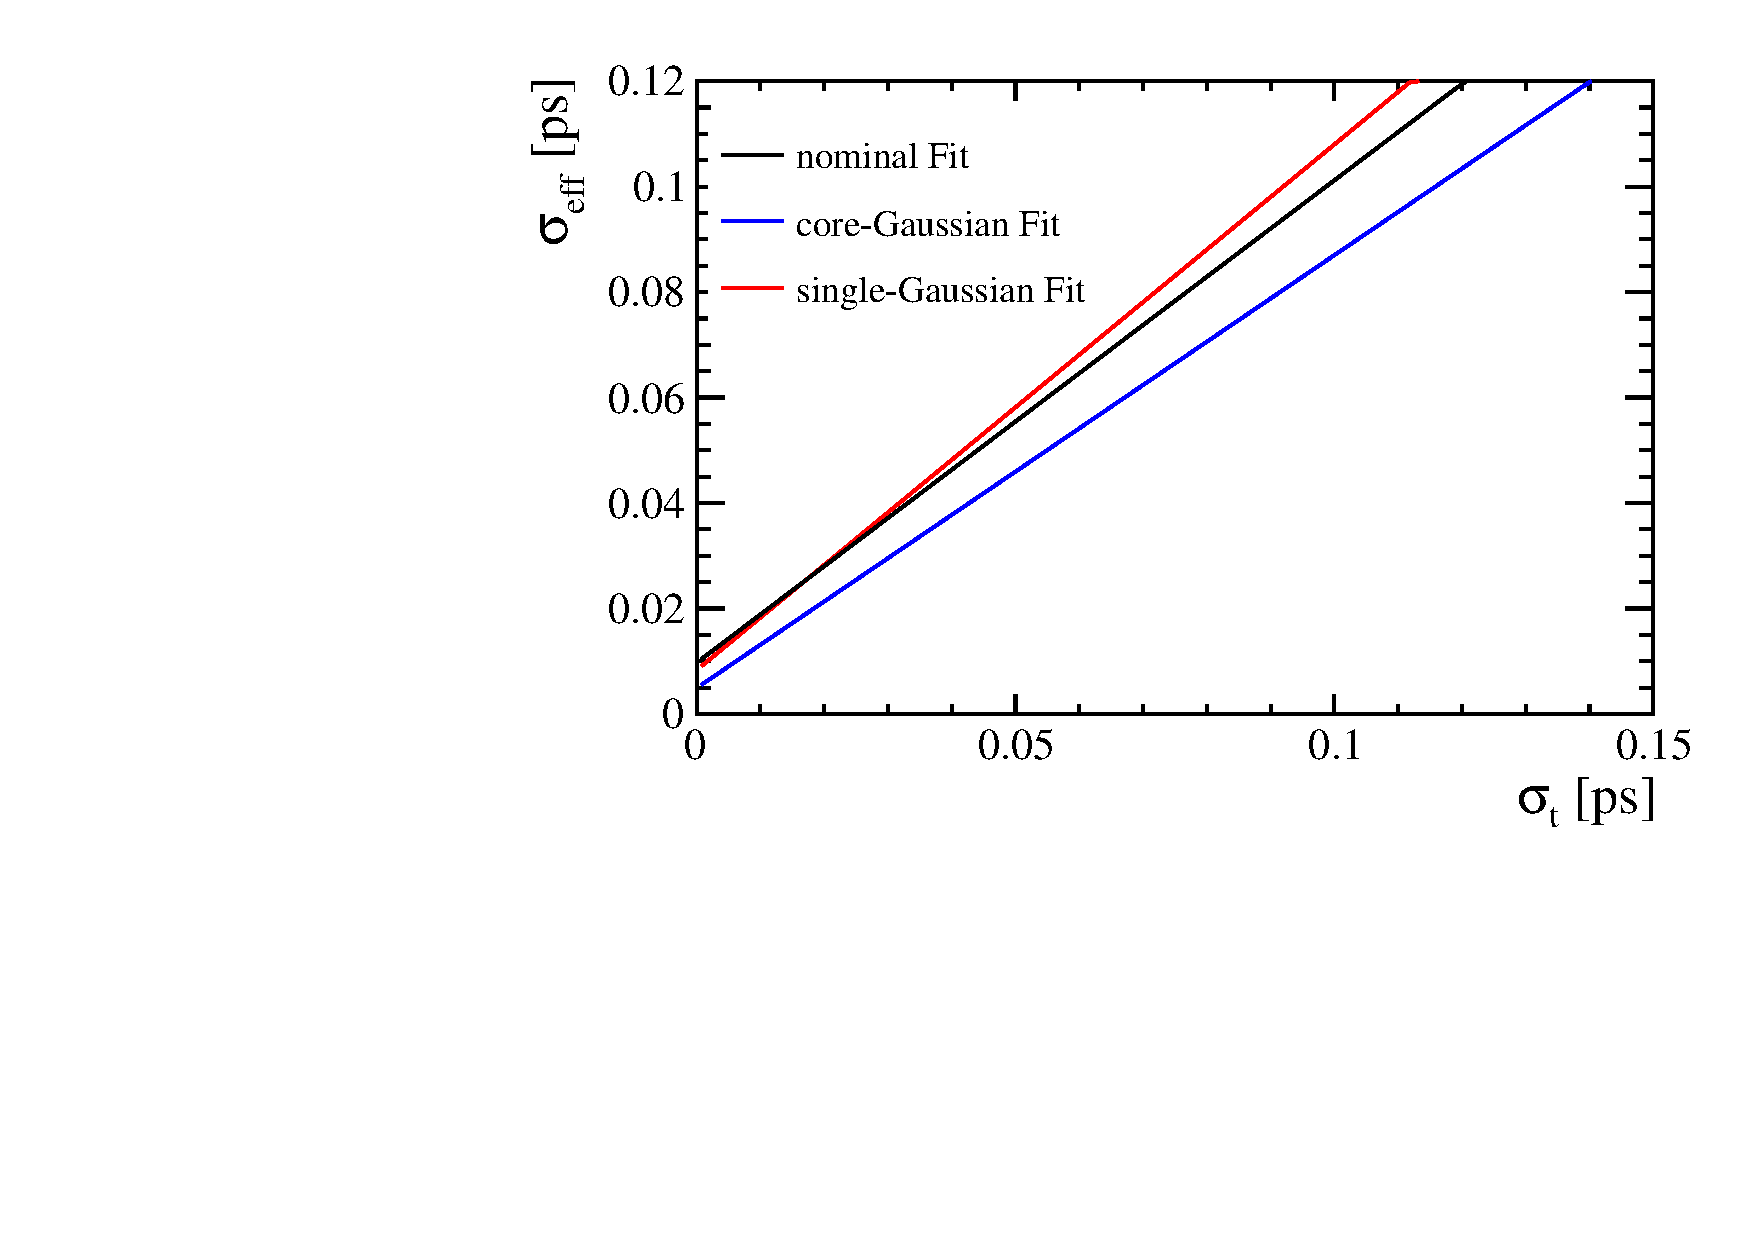
\includegraphics[height=!,width=0.6\textwidth]{figs/Resolution/ResoSyst.pdf}
\caption{\small The measured resolution scaling function of the per-event decay time error estimate $\sigma_t$ for fake $B_s$ candidates (Run-II data) 
for (black line) the nominal scaling, (blue line) only using the narrow gaussian width of the double gaussian fit model or (red line) when determining the resolution using a single gaussian model.}
\label{fig:SystscaleFactor}
\end{figure}


\subsection{Production, detection asymmetries and mixing frequency}

The systematic from the production, detection asymmetries and $\Delta m_s$ (in case of  $B_s \to D_s K \pi\pi$ decays) which are fixed in the fit
are evaluated by means of a toy study similar to the procedure performed for the time-acceptance. The parameters are assumed to be uncorrelated.

\subsection{Multiple candidates}

The fraction of events with multiple candidates has been found to be very small, it is $1.6\%$ for $D_s K \pi\pi$ and $1.5\%$ for $D_s \pi \pi\pi$. 
Thus the nominal result is obtained keeping all candidates, while a systematic uncertainty is assigned
by repeating the fit randomly keeping only one candidate when multiple ones are founds.
No shifts in the fit central values are observed.

\subsection{Length and momentum scales}
The uncertainty on the LHCb length scale is estimated to be at most $0.020\%$\cite{LHCb-ANA-2012-053}, which translates
directly in an uncertainty on $\Delta m_s$ of $0.020\%$ with other parameters being unaffected.
The momentum scale uncertainty is at most $0.022\%$.


\subsection{Phase space acceptance}

For the phase space acceptance we rely on simulated data.
The integration error due to the limited size of the MC sample 
used to normalize the signal PDF is evaluated by bootstrapping the MC sample and repeating the full time-dependent amplitude fit.

To asses the uncertainty due to possible data-simulation differences, we determine
alternative phase space efficiencies by varying the selection requirements on quantities that
are expected not to be well described by the simulation. 
In particular, we consider the following variations:

\begin{itemize}

	\item No BDT cut is applied
	
	\item A tighter BDT requirement is used (BDTG $> 0.6$)
	
%	\item The MC sample is reweighted to match the $p_T$ and $\eta$ distribution of the $B_s$ 
	
	\item No reweighting is applied 
	
	\item Instead of the PID responses obtained from the \textsf{PIDCorr} tool, we use the \textsf{PIDGen} tool to resample the PID variables \cite{LHCb-INT-2017-007}
	
	\item The raw MC PID variables are used
	
	\item Candidates with \textsf{BKGCAT}$=60$ are removed
	
\end{itemize}
We assign the sample variance of the fitted values using the alternative phase space acceptances as systematic.
\pretextcomment{
	This will be done when the final MC samples are available. 
	We expect the integration error to be negligible and the systematic error from data-simulation differences to be small.
	At the moment we estimate a systematic by assuming a flat phase space acceptance. 
	The resulting uncertainties shown in Table \ref{tab:sigSys2} should be considered as upper limit and illustrate that we are not highly sensitive 
	to the details of the phase space acceptance shape.
}

\subsection{Resonance description}

The following alternative line shape parameterizations are considered as part of the systematic studies:
\begin{itemize}

	\item The Lass description for the $K\pi$ $S$-wave is replaced by a relativistic Breit-Wigner propagator (Equation \ref{eq:gamma2})
	\item The Gounaris-Sakurai description for the $\rho(770)$ is replaced by a relativistic Breit-Wigner propagator (Equation \ref{eq:gamma2})
	\item The $\omega$ contribution to the decay channel $K_1(1270) \to K \, \rho(770)/\omega$ is set to zero
	\item For the decay channel $K^{*}(1410) \to K \, \rho(770)$, we include $\rho(770)-\omega$ mixing with a relative magnitude and phase determined from data
	\item Instead of taking the energy-dependent widths of the three-body resonances from Refs.~\cite{dArgent:2017gzv,Aaij:2017kbo}, we derive them from Equation~\ref{eq:gamma3} assuming an uniform phase space population. 

\end{itemize}
The data fits are repeated for each alternative model and the shifts of the central values are taken as systematic uncertainties. They are added in quadrature.

The uncertainties due to fixed masses and widths of resonances are evaluated
from toys where we vary them one-by-one within their quoted errors. 
In our nominal fit, the Blatt-Weisskopf radial parameter is set to $r_{BW}=1.5 \gev^{-1}$. 
Again, toys are generated according to this nominal configuration 
and then fitted whereby the radial parameter is uniformly varied within the interval $[0,3] \gev^{-1}$.


\subsection{Alternative amplitude models}

We tested several modifications of the LASSO model to assign an additional model uncertainty to the measured observables $r,\delta$ and $\gamma-2\beta_s$ as well as to 
the measured masses and widths of the $K_1(1400)$ and $K^*(1410)$ resonances.
The amplitude coefficients are by definition parameters of a given model which is why we do not evaluate a model uncertainty for them.
	
\begin{itemize}

	\item All amplitudes selected by Stage 1 of the model selection are included for both $b\to c$ and $b\to u$ transitions
				
	\item The decay channel $K_1(1270)[D] \to K^*(892) \, \pi$ is added where the $K^*(892) \, \pi$ system is in relative a D-wave state

	\item The decay channel $K_1(1400) \to K \, \rho(770)$ is added
	
	\item The decay channels $K_2^*(1430) \to K \, \rho(770)$ and $K_2^*(1430) \to K^*(892) \, \pi$ are added
	
	\item The decay channels $K(1460) \to K \, \rho(770)$ and $K(1460) \to K \, \sigma$ are added
	
	\item The $K(1460)$ resonance is removed
	
	\item The decay channels $K^*(1680) \to K \, \rho(770)$ and $K^*(1680) \to K^*(892) \, \pi$ are added
	
	\item The decay channels $K_2(1770) \to K \, \rho(770)$ and $K_2(1770)  \to K^*(892) \, \pi$ are added
		
	\item The amplitudes $B_s \to (D_s \, \pi)_{P} \, K^{*}(892)$ and $B_s \to (D_s \, K)_{P} \, \rho(770)$ are replaced by 
		$B_s \to (D_s \, \pi)_{S} \, K^{*}(892)$ and $B_s \to (D_s \, K)_{S} \, \rho(770)$
	
	\item Higher orbital angular momentum states are added for the amplitudes: $B_s[S,P,D] \to (D_s \, \pi)_{P} \, K^{*}(892)$ and $B_s[S,P,D] \to (D_s \, K)_{P} \, \rho(770)$
	
	\item The amplitudes $B_s \to (D_s \, \pi)_{P} \, K^{*}(892)$ and $B_s \to (D_s \, K)_{P} \, \rho(770)$ are removed

	\item The amplitudes $B_s \to (D_s \, K)_{P} \, \sigma$, $B_s \to (D_s \, K)_{P} \, f_2(1270)$ and $B_s \to (D_s \, K)_{P} \, f_0(1370)$ are added

	\item The amplitudes $B_s \to (D_s \, \pi)_{P} \, K_0^*(1430)$ and $B_s \to (D_s \, K)_{S} \, K_2^*(1430)$ are added

\end{itemize}
%
In total 20 different sets of amplitudes are fitted. In some cases, the fit fractions of additionally added amplitudes turn out to be exactly zero.
These model are effectively not distinguisbale from the baseline LASSO model and are not considered further.
From the remaining 15 models, we compute the sample variance for each observable and take it as model uncertainty.

%\subsection{Summary of systematic uncertainties}
%
%All contributing systematic uncertainties are summarized in Table \ref{tab:SystSummary}. 
%The individual uncertainties are summed in quadrature to arrive at the total systematic uncertainty for the respective CP observable.
%Their total magnitude ranges from (30-40)$\%$ of the statistical uncertainty of the fit.
\clearpage

\begin{sidewaystable}[h]
\centering
\caption{Systematic uncertainties on the fit parameters of the fit to $B_s \to D_s \pi \pi \pi$ data in units of statistical standard deviations.}
\resizebox{0.75\linewidth}{!}{
	\renewcommand{\arraystretch}{1.5}
	\begin{tabular}{l  c  c  c  c  c  c  c  c  c  c  c  | c }
\hline
\hline
Fit Parameter & Fit bias & Time-Acc. & Resolution & $\Delta m_{s}$ & Asymmetries & Background & Lineshapes & Resonances $m,\Gamma$ & Form-Factors & Phsp-Acc. & Amp. Model &  Total  \\ 
\hline
$B_s \to D_s \, ( K_1(1270) \to K^{*}(892) \, \pi ) \, \text{Mag}$ & 0.10 & 0.01 & 0.04 & 0.01 & 0.00 & 0.13 & 0.48 & 0.24 & 0.52 & 0.06 &  & 0.77 \\ 
$B_s \to D_s \, ( K_1(1270) \to K^{*}(892) \, \pi ) \, \text{Phase}$ & 0.07 & 0.01 & 0.04 & 0.01 & 0.01 & 0.08 & 0.35 & 0.28 & 0.34 & 0.12 &  & 0.58 \\ 
$B_s \to D_s \, ( K_1(1270) \to K^{*}_{0}(1430) \, \pi ) \, \text{Mag} $ & 0.04 & 0.01 & 0.01 & 0.00 & 0.00 & 0.24 & 1.44 & 0.11 & 0.17 & 0.04 &  & 1.47 \\ 
$B_s \to D_s \, ( K_1(1270) \to K^{*}_{0}(1430) \, \pi ) \, \text{Phase} $ & 0.04 & 0.01 & 0.02 & 0.01 & 0.00 & 0.19 & 5.83 & 0.19 & 0.61 & 0.09 &  & 5.87 \\ 
$B_s \to D_s \, ( K_1(1400) \to K^{*}(892) \, \pi ) \, \text{Mag} (b \to c)$ & 0.13 & 0.03 & 0.16 & 0.06 & 0.02 & 0.34 & 1.32 & 0.37 & 0.78 & 0.19 &  & 1.64 \\ 
$B_s \to D_s \, ( K_1(1400) \to K^{*}(892) \, \pi ) \, \text{Phase} (b \to c)$ & 0.14 & 0.02 & 0.09 & 0.02 & 0.01 & 0.18 & 0.54 & 0.26 & 0.40 & 0.08 &  & 0.77 \\ 
$B_s \to D_s \, ( K_1(1400) \to K^{*}(892) \, \pi ) \, \text{Mag} (b \to u)$ & 0.10 & 0.04 & 0.05 & 0.12 & 0.04 & 0.32 & 0.35 & 0.22 & 0.73 & 0.16 &  & 0.93 \\ 
$B_s \to D_s \, ( K_1(1400) \to K^{*}(892) \, \pi ) \, \text{Phase} (b \to u)$ & 0.02 & 0.04 & 0.04 & 0.10 & 0.03 & 0.08 & 0.79 & 0.21 & 0.31 & 0.08 &  & 0.89 \\ 
$B_s \to D_s \, ( K^{*}(1410) \to K^{*}(892) \, \pi ) \, \text{Mag} (b \to c)$ & 0.08 & 0.03 & 0.08 & 0.08 & 0.03 & 0.18 & 0.61 & 0.25 & 0.75 & 0.28 &  & 1.06 \\ 
$B_s \to D_s \, ( K^{*}(1410) \to K^{*}(892) \, \pi ) \, \text{Phase} (b \to c)$ & 0.35 & 0.01 & 0.06 & 0.01 & 0.01 & 0.13 & 0.60 & 0.19 & 0.68 & 0.08 &  & 1.00 \\ 
$B_s \to D_s \, ( K^{*}(1410) \to K \, \rho(770) ) \, \text{Mag}$ & 0.35 & 0.01 & 0.02 & 0.01 & 0.00 & 0.18 & 0.59 & 0.12 & 0.34 & 0.06 &  & 0.79 \\ 
$B_s \to D_s \, ( K^{*}(1410) \to K \, \rho(770) ) \, \text{Phase}$ & 0.18 & 0.00 & 0.01 & 0.01 & 0.00 & 0.24 & 0.34 & 0.09 & 0.21 & 0.06 &  & 0.51 \\ 
$B_s \to D_s \, ( K(1460) \to K^{*}(892) \, \pi ) \, \text{Mag} (b \to u)$ & 0.14 & 0.03 & 0.05 & 0.05 & 0.02 & 0.37 & 0.43 & 0.27 & 0.60 & 0.12 &  & 0.89 \\ 
$B_s \to D_s \, ( K(1460) \to K^{*}(892) \, \pi ) \, \text{Phase} (b \to u)$ & 0.13 & 0.04 & 0.11 & 0.07 & 0.03 & 0.21 & 0.84 & 0.49 & 0.46 & 0.06 &  & 1.11 \\ 
$B_s \to ( D_s \, \pi)_{P} \, \, K^{*}(892) \, \text{Mag} (b \to c)$ & 0.03 & 0.02 & 0.06 & 0.02 & 0.01 & 0.24 & 0.95 & 0.11 & 0.55 & 0.13 &  & 1.14 \\ 
$B_s \to ( D_s \, \pi)_{P} \, \, K^{*}(892) \, \text{Phase} (b \to c)$ & 0.20 & 0.01 & 0.13 & 0.02 & 0.01 & 0.51 & 1.10 & 0.18 & 0.52 & 0.26 &  & 1.38 \\ 
$B_s \to ( D_s \, \pi)_{P} \, \, K^{*}(892) \, \text{Mag} (b \to u)$ & 0.14 & 0.04 & 0.07 & 0.06 & 0.02 & 0.11 & 0.78 & 0.24 & 0.54 & 0.17 &  & 1.01 \\ 
$B_s \to ( D_s \, \pi)_{P} \, \, K^{*}(892) \, \text{Phase} (b \to u)$ & 0.24 & 0.05 & 0.19 & 0.06 & 0.03 & 0.47 & 1.54 & 0.28 & 0.59 & 0.17 &  & 1.77 \\ 
$B_s \to ( D_s \, K)_{P} \, \, \rho(770) \, \text{Mag} (b \to u)$ & 0.35 & 0.04 & 0.02 & 0.05 & 0.02 & 0.25 & 0.75 & 0.31 & 0.60 & 0.06 &  & 1.10 \\ 
$B_s \to ( D_s \, K)_{P} \, \, \rho(770) \, \text{Phase} (b \to u)$ & 0.12 & 0.03 & 0.05 & 0.06 & 0.02 & 0.68 & 0.50 & 0.38 & 0.66 & 0.08 &  & 1.14 \\ 
$m_{K_1(1400)} $ & 0.09 & 0.01 & 0.08 & 0.01 & 0.00 & 0.14 & 0.21 & 0.13 & 0.37 & 0.09 & 0.72 & 0.87 \\ 
$\Gamma_{K_1(1400)}$ & 0.01 & 0.01 & 0.01 & 0.02 & 0.01 & 0.14 & 0.46 & 0.13 & 0.44 & 0.10 & 0.62 & 0.91 \\ 
$m_{K^{*}(1410)}$ & 0.05 & 0.01 & 0.02 & 0.01 & 0.00 & 0.08 & 0.26 & 0.04 & 1.29 & 0.12 & 0.67 & 1.49 \\ 
$\Gamma_{K^{*}(1410)}$ & 0.25 & 0.00 & 0.02 & 0.01 & 0.00 & 0.14 & 0.15 & 0.04 & 1.40 & 0.07 & 0.72 & 1.61 \\ 
$r$ & 0.11 & 0.05 & 0.09 & 0.12 & 0.03 & 0.47 & 0.74 & 0.12 & 0.26 & 0.12 & 0.79 & 1.23 \\ 
$\delta$ & 0.19 & 0.04 & 0.07 & 0.10 & 0.05 & 0.10 & 0.29 & 0.03 & 0.11 & 0.02 & 0.52 & 0.66 \\ 
$\gamma - 2 \beta_{s}$ & 0.10 & 0.06 & 0.12 & 0.06 & 0.02 & 0.12 & 0.27 & 0.03 & 0.10 & 0.03 & 0.39 & 0.53 \\ 
\hline
\hline
\end{tabular}

}
\label{tab:normSys}
\end{sidewaystable}

\begin{table}[h]
\centering
\caption{Systematic uncertainties on the fit parameters of the phase-space integrated fit to $B_s \to D_s K\pi \pi$ data in units of statistical standard deviations.}
\resizebox{\linewidth}{!}{
	\renewcommand{\arraystretch}{1.5}
	\begin{tabular}{l  c  c  c  c  c  c  c  c  c  c  c  | c }
\hline
\hline
Fit Parameter & Fit bias & Time-Acc. & Resolution & $\Delta m_{s}$ & Asymmetries & Background & Lineshapes & Resonances $m,\Gamma$ & Form-Factors & Phsp-Acc. & Amp. Model &  Total  \\ 
\hline
$B_s \to D_s \, ( K_1(1270) \to K^{*}(892) \, \pi ) \, \text{Mag}$ & 0.10 & 0.01 & 0.04 & 0.01 & 0.00 & 0.13 & 0.48 & 0.24 & 0.52 & 0.06 &  & 0.77 \\ 
$B_s \to D_s \, ( K_1(1270) \to K^{*}(892) \, \pi ) \, \text{Phase}$ & 0.07 & 0.01 & 0.04 & 0.01 & 0.01 & 0.08 & 0.35 & 0.28 & 0.34 & 0.12 &  & 0.58 \\ 
$B_s \to D_s \, ( K_1(1270) \to K^{*}_{0}(1430) \, \pi ) \, \text{Mag} $ & 0.04 & 0.01 & 0.01 & 0.00 & 0.00 & 0.24 & 1.44 & 0.11 & 0.17 & 0.04 &  & 1.47 \\ 
$B_s \to D_s \, ( K_1(1270) \to K^{*}_{0}(1430) \, \pi ) \, \text{Phase} $ & 0.04 & 0.01 & 0.02 & 0.01 & 0.00 & 0.19 & 5.83 & 0.19 & 0.61 & 0.09 &  & 5.87 \\ 
$B_s \to D_s \, ( K_1(1400) \to K^{*}(892) \, \pi ) \, \text{Mag} (b \to c)$ & 0.13 & 0.03 & 0.16 & 0.06 & 0.02 & 0.34 & 1.32 & 0.37 & 0.78 & 0.19 &  & 1.64 \\ 
$B_s \to D_s \, ( K_1(1400) \to K^{*}(892) \, \pi ) \, \text{Phase} (b \to c)$ & 0.14 & 0.02 & 0.09 & 0.02 & 0.01 & 0.18 & 0.54 & 0.26 & 0.40 & 0.08 &  & 0.77 \\ 
$B_s \to D_s \, ( K_1(1400) \to K^{*}(892) \, \pi ) \, \text{Mag} (b \to u)$ & 0.10 & 0.04 & 0.05 & 0.12 & 0.04 & 0.32 & 0.35 & 0.22 & 0.73 & 0.16 &  & 0.93 \\ 
$B_s \to D_s \, ( K_1(1400) \to K^{*}(892) \, \pi ) \, \text{Phase} (b \to u)$ & 0.02 & 0.04 & 0.04 & 0.10 & 0.03 & 0.08 & 0.79 & 0.21 & 0.31 & 0.08 &  & 0.89 \\ 
$B_s \to D_s \, ( K^{*}(1410) \to K^{*}(892) \, \pi ) \, \text{Mag} (b \to c)$ & 0.08 & 0.03 & 0.08 & 0.08 & 0.03 & 0.18 & 0.61 & 0.25 & 0.75 & 0.28 &  & 1.06 \\ 
$B_s \to D_s \, ( K^{*}(1410) \to K^{*}(892) \, \pi ) \, \text{Phase} (b \to c)$ & 0.35 & 0.01 & 0.06 & 0.01 & 0.01 & 0.13 & 0.60 & 0.19 & 0.68 & 0.08 &  & 1.00 \\ 
$B_s \to D_s \, ( K^{*}(1410) \to K \, \rho(770) ) \, \text{Mag}$ & 0.35 & 0.01 & 0.02 & 0.01 & 0.00 & 0.18 & 0.59 & 0.12 & 0.34 & 0.06 &  & 0.79 \\ 
$B_s \to D_s \, ( K^{*}(1410) \to K \, \rho(770) ) \, \text{Phase}$ & 0.18 & 0.00 & 0.01 & 0.01 & 0.00 & 0.24 & 0.34 & 0.09 & 0.21 & 0.06 &  & 0.51 \\ 
$B_s \to D_s \, ( K(1460) \to K^{*}(892) \, \pi ) \, \text{Mag} (b \to u)$ & 0.14 & 0.03 & 0.05 & 0.05 & 0.02 & 0.37 & 0.43 & 0.27 & 0.60 & 0.12 &  & 0.89 \\ 
$B_s \to D_s \, ( K(1460) \to K^{*}(892) \, \pi ) \, \text{Phase} (b \to u)$ & 0.13 & 0.04 & 0.11 & 0.07 & 0.03 & 0.21 & 0.84 & 0.49 & 0.46 & 0.06 &  & 1.11 \\ 
$B_s \to ( D_s \, \pi)_{P} \, \, K^{*}(892) \, \text{Mag} (b \to c)$ & 0.03 & 0.02 & 0.06 & 0.02 & 0.01 & 0.24 & 0.95 & 0.11 & 0.55 & 0.13 &  & 1.14 \\ 
$B_s \to ( D_s \, \pi)_{P} \, \, K^{*}(892) \, \text{Phase} (b \to c)$ & 0.20 & 0.01 & 0.13 & 0.02 & 0.01 & 0.51 & 1.10 & 0.18 & 0.52 & 0.26 &  & 1.38 \\ 
$B_s \to ( D_s \, \pi)_{P} \, \, K^{*}(892) \, \text{Mag} (b \to u)$ & 0.14 & 0.04 & 0.07 & 0.06 & 0.02 & 0.11 & 0.78 & 0.24 & 0.54 & 0.17 &  & 1.01 \\ 
$B_s \to ( D_s \, \pi)_{P} \, \, K^{*}(892) \, \text{Phase} (b \to u)$ & 0.24 & 0.05 & 0.19 & 0.06 & 0.03 & 0.47 & 1.54 & 0.28 & 0.59 & 0.17 &  & 1.77 \\ 
$B_s \to ( D_s \, K)_{P} \, \, \rho(770) \, \text{Mag} (b \to u)$ & 0.35 & 0.04 & 0.02 & 0.05 & 0.02 & 0.25 & 0.75 & 0.31 & 0.60 & 0.06 &  & 1.10 \\ 
$B_s \to ( D_s \, K)_{P} \, \, \rho(770) \, \text{Phase} (b \to u)$ & 0.12 & 0.03 & 0.05 & 0.06 & 0.02 & 0.68 & 0.50 & 0.38 & 0.66 & 0.08 &  & 1.14 \\ 
$m_{K_1(1400)} $ & 0.09 & 0.01 & 0.08 & 0.01 & 0.00 & 0.14 & 0.21 & 0.13 & 0.37 & 0.09 & 0.72 & 0.87 \\ 
$\Gamma_{K_1(1400)}$ & 0.01 & 0.01 & 0.01 & 0.02 & 0.01 & 0.14 & 0.46 & 0.13 & 0.44 & 0.10 & 0.62 & 0.91 \\ 
$m_{K^{*}(1410)}$ & 0.05 & 0.01 & 0.02 & 0.01 & 0.00 & 0.08 & 0.26 & 0.04 & 1.29 & 0.12 & 0.67 & 1.49 \\ 
$\Gamma_{K^{*}(1410)}$ & 0.25 & 0.00 & 0.02 & 0.01 & 0.00 & 0.14 & 0.15 & 0.04 & 1.40 & 0.07 & 0.72 & 1.61 \\ 
$r$ & 0.11 & 0.05 & 0.09 & 0.12 & 0.03 & 0.47 & 0.74 & 0.12 & 0.26 & 0.12 & 0.79 & 1.23 \\ 
$\delta$ & 0.19 & 0.04 & 0.07 & 0.10 & 0.05 & 0.10 & 0.29 & 0.03 & 0.11 & 0.02 & 0.52 & 0.66 \\ 
$\gamma - 2 \beta_{s}$ & 0.10 & 0.06 & 0.12 & 0.06 & 0.02 & 0.12 & 0.27 & 0.03 & 0.10 & 0.03 & 0.39 & 0.53 \\ 
\hline
\hline
\end{tabular}

}
\label{tab:sigSys}
\end{table}


\begin{sidewaystable}[h]
\centering
\caption{Systematic uncertainties on the fit parameters of the full time-dependent amplitude fit to $B_s \to D_s K\pi \pi$ data in units of statistical standard deviations.}
\resizebox{\linewidth}{!}{
	\renewcommand{\arraystretch}{1.5}
	\begin{tabular}{l  c  c  c  c  c  c  c  c  c  c  c  | c }
\hline
\hline
Fit Parameter & Fit bias & Time-Acc. & Resolution & $\Delta m_{s}$ & Asymmetries & Background & Lineshapes & Resonances $m,\Gamma$ & Form-Factors & Phsp-Acc. & Amp. Model &  Total  \\ 
\hline
$B_s \to D_s \, ( K_1(1270) \to K^{*}(892) \, \pi ) \, \text{Mag}$ & 0.10 & 0.01 & 0.04 & 0.01 & 0.00 & 0.13 & 0.48 & 0.24 & 0.52 & 0.06 &  & 0.77 \\ 
$B_s \to D_s \, ( K_1(1270) \to K^{*}(892) \, \pi ) \, \text{Phase}$ & 0.07 & 0.01 & 0.04 & 0.01 & 0.01 & 0.08 & 0.35 & 0.28 & 0.34 & 0.12 &  & 0.58 \\ 
$B_s \to D_s \, ( K_1(1270) \to K^{*}_{0}(1430) \, \pi ) \, \text{Mag} $ & 0.04 & 0.01 & 0.01 & 0.00 & 0.00 & 0.24 & 1.44 & 0.11 & 0.17 & 0.04 &  & 1.47 \\ 
$B_s \to D_s \, ( K_1(1270) \to K^{*}_{0}(1430) \, \pi ) \, \text{Phase} $ & 0.04 & 0.01 & 0.02 & 0.01 & 0.00 & 0.19 & 5.83 & 0.19 & 0.61 & 0.09 &  & 5.87 \\ 
$B_s \to D_s \, ( K_1(1400) \to K^{*}(892) \, \pi ) \, \text{Mag} (b \to c)$ & 0.13 & 0.03 & 0.16 & 0.06 & 0.02 & 0.34 & 1.32 & 0.37 & 0.78 & 0.19 &  & 1.64 \\ 
$B_s \to D_s \, ( K_1(1400) \to K^{*}(892) \, \pi ) \, \text{Phase} (b \to c)$ & 0.14 & 0.02 & 0.09 & 0.02 & 0.01 & 0.18 & 0.54 & 0.26 & 0.40 & 0.08 &  & 0.77 \\ 
$B_s \to D_s \, ( K_1(1400) \to K^{*}(892) \, \pi ) \, \text{Mag} (b \to u)$ & 0.10 & 0.04 & 0.05 & 0.12 & 0.04 & 0.32 & 0.35 & 0.22 & 0.73 & 0.16 &  & 0.93 \\ 
$B_s \to D_s \, ( K_1(1400) \to K^{*}(892) \, \pi ) \, \text{Phase} (b \to u)$ & 0.02 & 0.04 & 0.04 & 0.10 & 0.03 & 0.08 & 0.79 & 0.21 & 0.31 & 0.08 &  & 0.89 \\ 
$B_s \to D_s \, ( K^{*}(1410) \to K^{*}(892) \, \pi ) \, \text{Mag} (b \to c)$ & 0.08 & 0.03 & 0.08 & 0.08 & 0.03 & 0.18 & 0.61 & 0.25 & 0.75 & 0.28 &  & 1.06 \\ 
$B_s \to D_s \, ( K^{*}(1410) \to K^{*}(892) \, \pi ) \, \text{Phase} (b \to c)$ & 0.35 & 0.01 & 0.06 & 0.01 & 0.01 & 0.13 & 0.60 & 0.19 & 0.68 & 0.08 &  & 1.00 \\ 
$B_s \to D_s \, ( K^{*}(1410) \to K \, \rho(770) ) \, \text{Mag}$ & 0.35 & 0.01 & 0.02 & 0.01 & 0.00 & 0.18 & 0.59 & 0.12 & 0.34 & 0.06 &  & 0.79 \\ 
$B_s \to D_s \, ( K^{*}(1410) \to K \, \rho(770) ) \, \text{Phase}$ & 0.18 & 0.00 & 0.01 & 0.01 & 0.00 & 0.24 & 0.34 & 0.09 & 0.21 & 0.06 &  & 0.51 \\ 
$B_s \to D_s \, ( K(1460) \to K^{*}(892) \, \pi ) \, \text{Mag} (b \to u)$ & 0.14 & 0.03 & 0.05 & 0.05 & 0.02 & 0.37 & 0.43 & 0.27 & 0.60 & 0.12 &  & 0.89 \\ 
$B_s \to D_s \, ( K(1460) \to K^{*}(892) \, \pi ) \, \text{Phase} (b \to u)$ & 0.13 & 0.04 & 0.11 & 0.07 & 0.03 & 0.21 & 0.84 & 0.49 & 0.46 & 0.06 &  & 1.11 \\ 
$B_s \to ( D_s \, \pi)_{P} \, \, K^{*}(892) \, \text{Mag} (b \to c)$ & 0.03 & 0.02 & 0.06 & 0.02 & 0.01 & 0.24 & 0.95 & 0.11 & 0.55 & 0.13 &  & 1.14 \\ 
$B_s \to ( D_s \, \pi)_{P} \, \, K^{*}(892) \, \text{Phase} (b \to c)$ & 0.20 & 0.01 & 0.13 & 0.02 & 0.01 & 0.51 & 1.10 & 0.18 & 0.52 & 0.26 &  & 1.38 \\ 
$B_s \to ( D_s \, \pi)_{P} \, \, K^{*}(892) \, \text{Mag} (b \to u)$ & 0.14 & 0.04 & 0.07 & 0.06 & 0.02 & 0.11 & 0.78 & 0.24 & 0.54 & 0.17 &  & 1.01 \\ 
$B_s \to ( D_s \, \pi)_{P} \, \, K^{*}(892) \, \text{Phase} (b \to u)$ & 0.24 & 0.05 & 0.19 & 0.06 & 0.03 & 0.47 & 1.54 & 0.28 & 0.59 & 0.17 &  & 1.77 \\ 
$B_s \to ( D_s \, K)_{P} \, \, \rho(770) \, \text{Mag} (b \to u)$ & 0.35 & 0.04 & 0.02 & 0.05 & 0.02 & 0.25 & 0.75 & 0.31 & 0.60 & 0.06 &  & 1.10 \\ 
$B_s \to ( D_s \, K)_{P} \, \, \rho(770) \, \text{Phase} (b \to u)$ & 0.12 & 0.03 & 0.05 & 0.06 & 0.02 & 0.68 & 0.50 & 0.38 & 0.66 & 0.08 &  & 1.14 \\ 
$m_{K_1(1400)} $ & 0.09 & 0.01 & 0.08 & 0.01 & 0.00 & 0.14 & 0.21 & 0.13 & 0.37 & 0.09 & 0.72 & 0.87 \\ 
$\Gamma_{K_1(1400)}$ & 0.01 & 0.01 & 0.01 & 0.02 & 0.01 & 0.14 & 0.46 & 0.13 & 0.44 & 0.10 & 0.62 & 0.91 \\ 
$m_{K^{*}(1410)}$ & 0.05 & 0.01 & 0.02 & 0.01 & 0.00 & 0.08 & 0.26 & 0.04 & 1.29 & 0.12 & 0.67 & 1.49 \\ 
$\Gamma_{K^{*}(1410)}$ & 0.25 & 0.00 & 0.02 & 0.01 & 0.00 & 0.14 & 0.15 & 0.04 & 1.40 & 0.07 & 0.72 & 1.61 \\ 
$r$ & 0.11 & 0.05 & 0.09 & 0.12 & 0.03 & 0.47 & 0.74 & 0.12 & 0.26 & 0.12 & 0.79 & 1.23 \\ 
$\delta$ & 0.19 & 0.04 & 0.07 & 0.10 & 0.05 & 0.10 & 0.29 & 0.03 & 0.11 & 0.02 & 0.52 & 0.66 \\ 
$\gamma - 2 \beta_{s}$ & 0.10 & 0.06 & 0.12 & 0.06 & 0.02 & 0.12 & 0.27 & 0.03 & 0.10 & 0.03 & 0.39 & 0.53 \\ 
\hline
\hline
\end{tabular}

}
\label{tab:sigSys2}
\end{sidewaystable}

